% p10-03 例 2：△ABC ∠B=30°, AB=6, P 在 BC 上。求 PA + (1/2) PB 最小
% 在 B 处作射线 l'（远 A 侧）与 BC 成 30°；过 A 作 l' 的垂线，垂足 H0；最小值 = AH0 = 6 sin60° = 3√3
\documentclass[tikz,border=4pt]{standalone}
\usepackage{ctex}
\usepackage{amsmath}
\usetikzlibrary{calc, arrows.meta}
\begin{document}
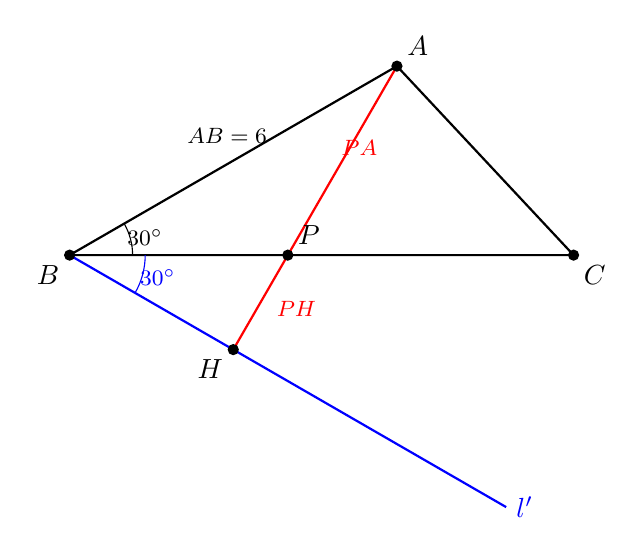
\begin{tikzpicture}[scale=0.8, thick]
  \coordinate (B) at (0, 0);
  \coordinate (C) at (8, 0);
  % A 使 ∠B=30°、AB=6：A = (6 cos30°, 6 sin30°) = (5.196, 3)
  \coordinate (A) at (5.196, 3);
  % l' 在 BC 下方，与 BC 成 30°：方向 (cos(-30°), sin(-30°))=(0.866, -0.5)
  \coordinate (Lend) at (6.93, -4.0);
  % 过 A(5.196, 3) 向 l' 作垂线，垂足 H0
  % 投影 t = A · dir = 5.196*0.866 + 3*(-0.5) = 4.5 - 1.5 = 3
  % H0 = 3 * (0.866, -0.5) = (2.598, -1.5)
  \coordinate (H0) at (2.598, -1.5);
  % P 取 AH0 与 BC 的交点（即 P 就是 BC 上的最优位置）
  % AH0 直线参数化：(5.196,3) + s((2.598,-1.5)-(5.196,3)) = (5.196 - 2.598s, 3 - 4.5s)；y=0 ⇒ s=2/3 ⇒ x=5.196-1.732=3.464
  \coordinate (P) at (3.464, 0);
  % P 到 l' 的垂足 H
  % 投影 t = 3.464*0.866 = 3.0；H = 3*(0.866, -0.5) = (2.598, -1.5) = H0! (因为 A, P, H0 共线 → A 在 l' 上的垂足 就是 P 在 l' 上的垂足？不对)
  % 让我重新计算 P 在 l' 上的垂足：投影 t_P = 3.464*0.866 + 0 = 3.0；位置 = 3.0*(0.866,-0.5) = (2.598,-1.5)
  % 巧合：P 在 l' 上的垂足就是 H0。是的，因为 AH0 ⊥ l'，AH0 与 BC 的交点 P 仍满足 PH0⊥l'。
  \coordinate (H) at (2.598, -1.5);

  \draw (A)--(B)--(C)--cycle;
  \draw[blue, thick] (B)--(Lend);
  \node[blue, right] at (Lend) {$l'$};

  \draw[red, thick] (A)--(P);
  \draw[red, thick] (P)--(H);

  \filldraw (A) circle (2pt) node[above right] {$A$};
  \filldraw (B) circle (2pt) node[below left] {$B$};
  \filldraw (C) circle (2pt) node[below right] {$C$};
  \filldraw (P) circle (2pt) node[above right] {$P$};
  \filldraw (H) circle (2pt) node[below left] {$H$};

  % 角标 30°
  \draw[blue, thin] (1.2, 0) arc[start angle=0, end angle=-30, radius=1.2];
  \node[blue, font=\footnotesize] at (1.4, -0.35) {$30^\circ$};
  % ∠B in triangle
  \draw[thin] (1.0, 0) arc[start angle=0, end angle=30, radius=1.0];
  \node[font=\footnotesize] at (1.2, 0.28) {$30^\circ$};

  \node[font=\footnotesize] at (2.5, 1.9) {\footnotesize $AB=6$};
  \node[red, font=\footnotesize] at (4.6, 1.7) {$PA$};
  \node[red, font=\footnotesize] at (3.6, -0.85) {$PH$};
\end{tikzpicture}
\end{document}
